\section{The Solenoid and the Steel Return Yoke}
\label{sec:solenoid}

The Compact Muon \emph{Solenoid} sports one of the world's most energetic solenoids and is paramount to the success of CMS.
Particles that exit the HCAL~\ref{subsec:hcal} arrive at the cylindrical magnet which is 12.5 \meter in length, has a bore diameter of 6.3 \meter when cold, and generates a uniform 3.8 \tesla magnetic field parallel to the beam line.
To generate such a large and uniform magnetic field, a current of 18,000 A travels through superconducting Nb-Ti coils inside the approximately 360 \meter$^3$ volume (Fig.~\ref{fig:cms_magnetic_field}).
This magnetic field is 100,000 times stronger than that of Earth's, as measured at the surface, and stores a massive 2.6 GJ of energy - approximately equivalent to the kinetic energy of an Airbus A320 in flight.
%%%%%%%%%%%%%%%%%%%%
\begin{figure}[pbth]
    \centering
    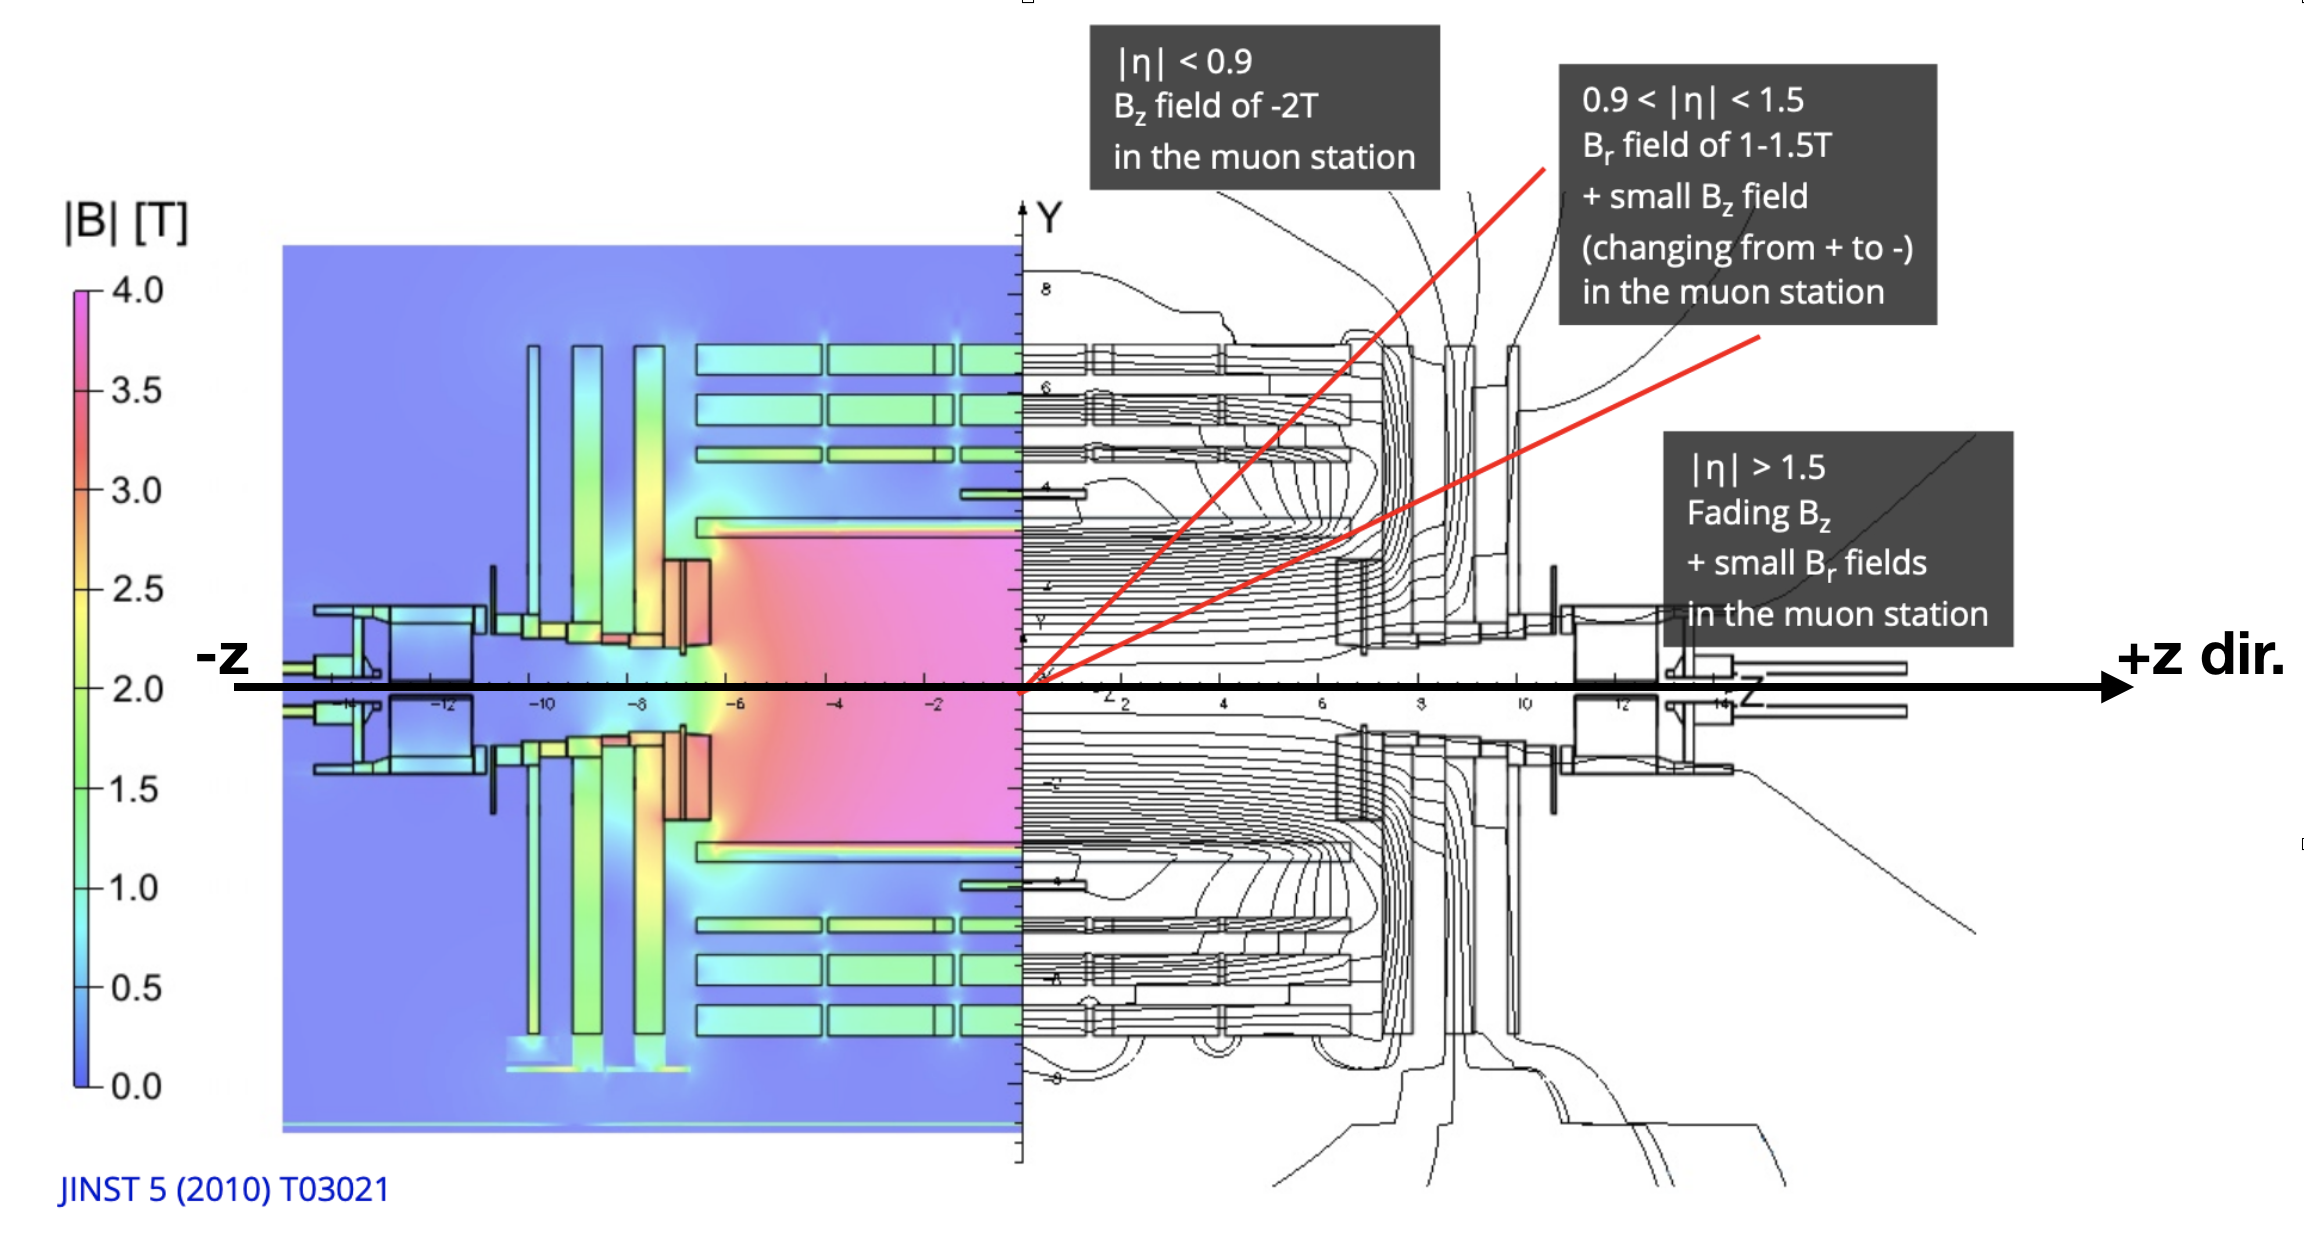
\includegraphics[width=15cm,height=15cm,keepaspectratio]{figures/cms/solenoid/CMS_longitudinal_view_magnetic_field.png}
        \caption{
        A longitudinal cross section of CMS showing the values of the magnetic field over the volume of CMS and various field lines. 
        The magnetic field reaches its maximum of 3.8 T in the center of the detector.}
        \label{fig:cms_magnetic_field}
    \end{figure}
    %%%%%%%%%%%%%%%%%%%%

% the direction in which the protons collide, which we call the z direction.
When charged particles travel through a magnetic field, a Lorentz force is applied to them, thereby separating out the particle tracks as they travel away from the interaction point.
The large magnetic field generated by CMS assists in The relative change in momentum (\ie the momentum resolution) is 
% As the charged particles bend out and away from the beam pipe, they pass through the silicon tracking system, which has excellent resolution ""
% Imagine CMS as a giant camera that takes a picture every few ns of the outgoing particles. 

\textbf{Steel Return Yoke:} 
Most of the mass of CMS comes from the \emph{steel return yoke} which helps to redirect the magnetic field back on itself. 
The yoke system constitutes 10,000 tonnes, which is 89\% of the total mass of CMS.
It is comprised of 5 wheels and 2 endcaps
